\chapter[Selected Applications Of Detection Proposals]{Selected Applications Of \newline Detection Proposals}
\label{chapter:applications}

In the final chapter of this thesis, we present two applications of our detection proposals method. The first is a end-to-end object detection pipeline that uses detection proposals at its core. The second is a simple tracking system that combines detection proposals and matching.

The purpose of this chapter is not to improve some specific state of the art, but to show that detection proposals can be used for different problems related to underwater robot perception, in the context of marine debris detection. We expect that the ideas presented in this chapter can be further developed to become state of the art in their respective sub-fields, with specific application to tasks related to collecting marine debris from the ocean floor.

\section{End-to-End Object Detection}

\subsection{Introduction}

We have built a object detection pipeline based on detection proposals. While object detection is a well researched subject, many underwater object detection systems suffer from generalization issues that we have mentioned in the past.

There is a rampart use of feature engineering that is problem and object specific, which harms the ability to use such features for different objects and environments. We have previously shown how classic methods for sonar images do not perform adequately for marine debris, and extensions to use deep neural networks are required.

A natural extension of our detection proposal system is to include a classification stage so full object detection can be performed. An additional desirable characteristic of a CNN-based object detector is end-to-end training. This consists of training a single network that perform both tasks (detection and classification) in a way that all intermediate steps are also internally learned by the network. Only input images and labels must be provided (hence end-to-end).

In this section we showcase a CNN architecture that can perform both object detection (through detection proposals) and object recognition (with a integrated classifier) in a single unified network. We do this using multi-task learning, where a CNN architecture is designed to output two sets of values: An objectness score for detection proposals (same as Chapter \ref{chapter:proposals}), and a softmax probability distribution over class labels (like our image classifiers in Chapter \ref{chapter:sonar-classification}).

We show that this architecture can be easily trained with only labeled image crops that contain both objectness and class labels, which effectively makes an end-to-end system with acceptable performance.

\subsection{Proposed Method}

We design a network that takes a single input image patch and produces two outputs, namely:

\begin{itemize}
	\item \textbf{Objectness}. This corresponds as an objectness score in $[0, 1]$ used to decide if an object is present in the image. Its interpretation is the same as with our detection proposals algorithm (in Chapter \ref{chapter:proposals}). The basic idea is to threshold the objectness score or use ranking to produce detections. This is implemented as a sigmoid activation function.
	\item \textbf{Class Decision}. This corresponds to one of $C + 1$ pre-defined classes, which indicate the object class decided by the network. We include an additional class that represents background, meaning no object present in that window. This is implemented as a softmax activation which produces a probability distribution over classes. The output class can then be selected by the one with highest probability.
\end{itemize}

Each output represents a different "task" in a multi-task learning framework \cite{ruder2017overview}. Objectness represents the task of object localization, while class decisions corresponds to the classification task.

The basic network design that we propose is shown in Figure \ref{apps-detection:basicArchitecture}. A certain number of convolutional feature maps form the "trunk" of the network, which are feed directly from the input image. A 1D feature vector is produced by the network trunk, typically by a fully connected layer receiving input from the convolutional feature maps, but we give freedom to the  network designer to set the right architecture for the problem.

It should be noted that the shared feature vector does not need to be one-dimensional. There is the possibility to keep two-dimensional convolutional feature maps in order to exploit spatial structure in the features. In order to produce a one-dimensional feature vector, flattening is usually applied, and this could lose some spatial information. We mention this option but do not explore it further.

Two output sub-networks are fed by the shared feature vector. One sub-network produces an objectness score, while the other sub-network produces a class decision. Once this network is built and trained, it can be used in a sliding window fashion over the input image to produce detections that also include class information, forming a complete object detection system.

The use of a shared feature vector is based on the idea of information sharing. As objectness and object classification share some similarities, such as the concept of an object and variability between object classes, it makes sense to learn a feature vector that combine/fuses both kinds of information into a single source.  This vector should encode both objectness and class information, allowing for a classifier and objectness regressor to extract useful information for each of the tasks.

Another view of the shared feature vector is that of minimizing the amount of information required for both tasks. As both tasks require common information, a smaller feature vector can be learned instead of learning two feature vectors that might be forced to duplicate information. This should require less data and a simpler network architecture.

There is also evidence \cite{caruana1997multitaskJournalML} that multi-task learning can improve the performance of each individual task . Rich Caruana's PhD thesis \cite{caruana1997multitask} was one of the first to study this topic, and his work found that performance improvements in multi-task learning come from extra information in the training signals of the additional tasks. There are different mechanisms that produce this effect: statistical data amplification, attribute selection, eavesdropping, and representation bias. Caruana also mentions that backpropagation automatically discovers how the tasks are related in a partially unsupervised way.

\newpage
State of the art object detection methods like Faster R-CNN \cite{ren2015faster} and YOLO \cite[1em]{redmon2016you} also use multi-task learning, and we recognize that we use similar ideas to build our object detector.
Our method could be considered a simplification of Faster R-CNN without bounding box regression and only a single anchor box, which allows for one scale only. In comparison, our method is trained end-to end, while Faster R-CNN and YOLO can only be trained successfully with a pre-trained network on the ImageNet dataset.

Figure \ref{apps-detection:classicNetRealization} represents our particular instantiation of the basic architecture fro Figure \ref{apps-detection:basicArchitecture}. This architecture is based on ClassicNet but with two "heads" for classification and object localization. We obtained this model by performing grid search on a validation set with a variation of number of layers, convolutional filters, and shared feature vector size.

\begin{figure}[!htb]
	\centering
	\begin{tikzpicture}[style={align=center, minimum height=0.5cm, minimum width = 2.5cm}]
	\node[] (dummy) {};
	\node[draw, left=0.0em of dummy] (objClassifier) {{\scriptsize Object Classifier}};
	\node[above=1em of objClassifier] (objClass) {{\scriptsize Object Class}};
	
	\node[draw, right=0.0em of dummy] (objDetector) {{\scriptsize Objectness Regressor}};
	\node[above=1em of objDetector] (obj) {{\scriptsize Objectness}};
	
	\node[draw, below=1em of dummy] (fc) {{\scriptsize Feature Vector}};
	
	\node[draw, below=1em of fc](conv) {\scriptsize{Convolutional Features}};
	\node[below=1em of conv](inputImage) {{\scriptsize Input Image}};
	\draw[-latex] (inputImage) -- (conv);
	\draw[-latex] (conv) -- (fc);
	\draw[-latex] (fc) -- (objDetector);
	\draw[-latex] (fc) -- (objClassifier);
	\draw[-latex] (objClassifier) -- (objClass);
	\draw[-latex] (objDetector) -- (obj);
	\end{tikzpicture}
	\caption[Basic Object Detection Architecture]{Basic Object Detection Architecture. A single image is input to a neural network with two outputs. A shared set of convolutional features are computed, producing a feature vector that is used by both the object classifier and object detector to produce their decisions.}
	\label{apps-detection:basicArchitecture}
\end{figure}


\begin{figure}[!htb]
	\centering
	\begin{tikzpicture}[style={align=center, minimum height=0.5cm, minimum width = 2.0cm}]
	\node[] (dummy) {};
	\node[draw, left=0.1em of dummy] (probsFc1) {{\scriptsize FC(96)}};
	\node[draw, above=1em of probsFc1] (probsFcOut) {{\scriptsize FC(\# of classes)}};
	\node[above=1em of probsFcOut] (probs) {{\scriptsize Class Probabilities}};
	
	\node[draw, right=0.1em of dummy] (objFc1) {{\scriptsize FC(96)}};
	\node[draw, above=1em of objFc1] (objFcOut) {{\scriptsize FC(1)}};
	\node[above=1em of objFcOut] (obj) {{\scriptsize Objectness}};
	
	\node[draw, below=1em of dummy] (fc1) {{\scriptsize FC(128)}};
	
	\node[draw, below=1em of fc1] (mp2) {{\scriptsize MaxPooling(2, 2)}};
	\node[draw, below=1em of mp2] (conv2) {{\scriptsize Conv($32$, $5 \times 5$)}};;
	\node[draw, below=1em of conv2] (mp1) {{\scriptsize MaxPooling(2, 2)}};
	\node[draw, below=1em of mp1](conv1) {{\scriptsize Conv($32$, $5 \times 5$)}};
	\node[below=1em of conv1](inputImage) {{\scriptsize $96 \times 96$ Input Image}};
	\draw[-latex] (inputImage) -- (conv1);
	\draw[-latex] (conv1) -- (mp1);
	\draw[-latex] (mp1) -- (conv2);
	\draw[-latex] (conv2) -- (mp2);
	\draw[-latex] (mp2) -- (fc1);
	\draw[-latex] (fc1) -- (objFc1);
	\draw[-latex] (objFc1) -- (objFcOut);
	\draw[-latex] (fc1) -- (probsFc1);
	\draw[-latex] (probsFc1) -- (probsFcOut);
	\draw[-latex] (probsFcOut) -- (probs);
	\draw[-latex] (objFcOut) -- (obj);
	\end{tikzpicture}
	\caption[Realization of the proposed architecture as a Convolutional Neural Network]{Realization of the proposed architecture as a Convolutional Neural Network. This CNN has 1.8 Million trainable weights.}
	\label{apps-detection:classicNetRealization}
\end{figure}

The network is trained end-to-end with both tasks of detection and recognition at the same time. This process requires the minimization of a multi-task loss function. In our case we use a linear combination of two loss terms. For classification we use the categorical cross-entropy loss, while for objectness we use the mean squared error:

\begin{equation}
	L(y, \hat{y}) = n^{-1} \sum (y_o - \hat{y}_o)^2 - \gamma \sum_i \sum_c y^c_i \log \hat{y}^c_i
	\label{apps-detection:multiTaskLoss}
\end{equation}

Where the $o$ subscript is used for objectness labels, and the $c$ superscript for class information. The factor $\gamma$ controls the importance of each sub-loss term into the overall loss value. Tuning an appropriate value is key to obtain good performance. We evaluate the effect of this parameter in our experiments.\\

Batch normalization \cite{ioffe2015batch} is used after every trainable layer to prevent overfitting and accelerate training. The network is trained with stochastic gradient descent with a batch size of $b = 128$ images and the ADAM optimizer \cite[1em]{kingma2014adam} with a starting learning rate of $\alpha = 0.01$. We train until the validation loss stops improving, normally after 20 epochs.

\subsection{Experimental Evaluation}

From the perspective of the Marine Debris task, an object detector has two main objectives: to detect debris objects with high recall, and to classify them with high accuracy. We evaluate recall instead of both precision and recall as the object detector has to generalize well outside of its training set, where it might detect novel objects but classify them incorrectly. To evaluate false positives, we measure the number of output proposals, as it correlates with the possibility of a false positive.

We evaluate our object detection method in terms of three metrics: proposal recall, classification accuracy, and number of output proposals. We use proposal recall as defined in Chapter \ref{chapter:proposals}, while we define classification accuracy for this problem as the ratio between correctly classified bounding boxes over the number of ground truth bounding boxes. This kind of evaluation metrics allow for separate assessment of object localization (detection) and classification.

For simplicity we only use objectness thresholding as a way to extract detections from objectness scores, as it was the best performing method when we evaluated it in Chapter \ref{chapter:proposals}. For many point-wise comparisons we use $T_o = 0.5$, as it makes sense since it is the middle value of the valid scale for $T_o$, and in general it produces a good trade-off between number of detection proposals and recall and accuracy.

We have not yet defined a concrete value of the multi-task loss weight $\gamma$. Most papers that use multi-task learning tune this value on a validation set, but we have found out that setting the right value is critical for good performance and balance between the tasks. We take an empiric approach and evaluate a predefined set of values, namely $\gamma \in [0.5, 1, 2, 3, 4]$ and later determine which produces the best result using both recall and accuracy. This is not an exhaustive evaluation, but we found that it produces good results. Recent research by Kendall et al. \cite[-6em]{kendall2017multi} proposes a method to automatically tune multi-task weights using task uncertainty that could be used in the future. This paper also notes that multi-task weights have a great effect on overall system performance.

Figure \ref{apps-detection:objectnessThreshVsAccuracyRecallAndNumberOfProposals} shows our principal results as the objectness threshold $T_o$ is varied and we also show the effect of different multi-task loss weight $\gamma$.

Our detection proposals recall is good, close to $95$ \% at $T_o = 0.5$ for many values of $\gamma$, showing little variation between different choices of that parameter. Larger variations in recall are observed for bigger ($> 0.6$) values of $T_o$.

Classification accuracy produced by our system shows a considerable variation across different values of the multi-task loss weight $\gamma$. The best performing value is $\gamma = 3$, but it is not clear why this value is optimal or how other values can be considered (other than trial and error). As mentioned before, setting multi-task loss weights is not trivial and has a large effect on the result. It is also counter-intuitive that a larger value of $gamma$ leads to lower classification performance. At $T_o = 0.5$, the best performing model produces $70$ \% accuracy.

Looking at the number of proposals, again there is a considerable variation between different values of $gamma$, but the number of proposal reduces considerably with an increasing objectness threshold $T_o$. For $T_o = 0.5$ the best performing value $gamma = 3$ produces $112 \pm 62$ proposals per image. This is higher than the number of proposals that our non-classification methods produce (as shown in Chapter \ref{chapter:proposals}).

From a multi-task learning point of view, learning the classification task seems to be considerably harder than the objectness regression task. This is probably due to the different task complexity (modeling class-agnostic objects seems to be easier than class-specific objects), and also we have to consider the limitations from our small training set. Other object detectors like Faster R-CNN are usually trained in much bigger datasets, also containing more object pose variability.

\begin{figure*}[t]
	\centering
	\forcerectofloat
	\begin{tikzpicture}
		\begin{axis}[height = 0.21\textheight, width = 0.49\textwidth, xlabel={Objectness Threshold ($T_o$)}, ylabel={Detection Recall (\%)}, xmin=0, xmax=1.0, ymin=0, ymax=100.0, ymajorgrids=true, xmajorgrids=true, grid style=dashed, legend pos = south west]        
			\addplot+[mark=none, y filter/.code={\pgfmathparse{\pgfmathresult*100.}\pgfmathresult}] table[x  = threshold, y  = recall, col sep = space] {chapters/data/applications/detection/thresholdVsRecallAndAccuracyAtIoU0.5Lambda0.5.csv};
			\addplot+[mark=none, y filter/.code={\pgfmathparse{\pgfmathresult*100.}\pgfmathresult}] table[x  = threshold, y  = recall, col sep = space] {chapters/data/applications/detection/thresholdVsRecallAndAccuracyAtIoU0.5Lambda1.csv};
			\addplot+[mark=none, y filter/.code={\pgfmathparse{\pgfmathresult*100.}\pgfmathresult}] table[x  = threshold, y  = recall, col sep = space] {chapters/data/applications/detection/thresholdVsRecallAndAccuracyAtIoU0.5Lambda2.csv};
			\addplot+[mark=none, y filter/.code={\pgfmathparse{\pgfmathresult*100.}\pgfmathresult}] table[x  = threshold, y  = recall, col sep = space] {chapters/data/applications/detection/thresholdVsRecallAndAccuracyAtIoU0.5Lambda3.csv};
			\addplot+[mark=none, y filter/.code={\pgfmathparse{\pgfmathresult*100.}\pgfmathresult}] table[x  = threshold, y  = recall, col sep = space] {chapters/data/applications/detection/thresholdVsRecallAndAccuracyAtIoU0.5Lambda4.csv};
		\end{axis}        
	\end{tikzpicture}
	\begin{tikzpicture}
		\begin{axis}[height = 0.21\textheight, width = 0.49\textwidth, xlabel={Objectness Threshold ($T_o$)}, ylabel={Classification Accuracy (\%)}, xmin=0, xmax=1.0, ymin=0, ymax=100.0, ymajorgrids=true, xmajorgrids=true, grid style=dashed, legend pos = south west]        
			\addplot+[mark=none, y filter/.code={\pgfmathparse{\pgfmathresult*100.}\pgfmathresult}] table[x = threshold, y = accuracy, col sep = space] {chapters/data/applications/detection/thresholdVsRecallAndAccuracyAtIoU0.5Lambda0.5.csv};
			\addplot+[mark=none, y filter/.code={\pgfmathparse{\pgfmathresult*100.}\pgfmathresult}] table[x = threshold, y = accuracy, col sep = space] {chapters/data/applications/detection/thresholdVsRecallAndAccuracyAtIoU0.5Lambda1.csv};
			\addplot+[mark=none, y filter/.code={\pgfmathparse{\pgfmathresult*100.}\pgfmathresult}] table[x = threshold, y  = accuracy, col sep = space] {chapters/data/applications/detection/thresholdVsRecallAndAccuracyAtIoU0.5Lambda2.csv};
			\addplot+[mark=none, y filter/.code={\pgfmathparse{\pgfmathresult*100.}\pgfmathresult}] table[x = threshold, y = accuracy, col sep = space] {chapters/data/applications/detection/thresholdVsRecallAndAccuracyAtIoU0.5Lambda3.csv};
			\addplot+[mark=none, y filter/.code={\pgfmathparse{\pgfmathresult*100.}\pgfmathresult}] table[x = threshold, y = accuracy, col sep = space] {chapters/data/applications/detection/thresholdVsRecallAndAccuracyAtIoU0.5Lambda4.csv};
		\end{axis}        
	\end{tikzpicture}
	
	\begin{tikzpicture}
		\begin{axis}[height = 0.21\textheight, width = 0.49\textwidth, xlabel={Objectness Threshold ($T_o$)}, ylabel={Number of Proposals}, xmin=0, xmax=1.0, ymin=0, ymajorgrids=true, xmajorgrids=true, grid style=dashed, legend pos = outer north east]        
			\addplot+[mark=none] table[x  = threshold, y = numberOfProposals, col sep = space] {chapters/data/applications/detection/thresholdVsRecallAndAccuracyAtIoU0.5Lambda0.5.csv};
			\addlegendentry{$\gamma = \frac{1}{2}$}
			\addplot+[mark=none] table[x  = threshold, y = numberOfProposals, col sep = space] {chapters/data/applications/detection/thresholdVsRecallAndAccuracyAtIoU0.5Lambda1.csv};
			\addlegendentry{$\gamma = 1$}
			\addplot+[mark=none] table[x  = threshold, y = numberOfProposals, col sep = space] {chapters/data/applications/detection/thresholdVsRecallAndAccuracyAtIoU0.5Lambda2.csv};
			\addlegendentry{$\gamma = 2$}
			\addplot+[mark=none] table[x  = threshold, y = numberOfProposals, col sep = space] {chapters/data/applications/detection/thresholdVsRecallAndAccuracyAtIoU0.5Lambda3.csv};
			\addlegendentry{$\gamma = 3$}
			\addplot+[mark=none] table[x  = threshold, y = numberOfProposals, col sep = space] {chapters/data/applications/detection/thresholdVsRecallAndAccuracyAtIoU0.5Lambda4.csv};
			\addlegendentry{$\gamma = 4$}
		\end{axis}        
	\end{tikzpicture}
	\caption[Detection Recall, Classification Accuracy and Number of Proposals as a function of Objectness Threshold $T_o$]{Detection Recall, Classification Accuracy and Number of Proposals as a function of Objectness Threshold $T_o$. Different combinations of the multi-task loss weight $\gamma$ are shown.}
	\label{apps-detection:objectnessThreshVsAccuracyRecallAndNumberOfProposals}
\end{figure*}

Figure \ref{apps-detection:accuracyRecallVsNumberOfProposals} shows the relation between recall/accuracy and the number of detection proposals. For detection proposal recall, our results show that only 100 to 150 proposals per image are required to achieve $95$ \% recall, and using more proposals only marginally increases performance.

For classification accuracy, the pattern is different from proposal recall. As mentioned previously, there is a large variation in classification performance as the multi-task loss weight $\gamma$ is varied, and clearly $\gamma = 3$ performs best. But accuracy increases slowly as the number of proposals is increased, which shows that many proposals are being misclassified, indicating a problem with the classification branch of the network. We expected that classification performance will increase in a similar way as to proposal recall, if the network is performing well at both tasks, but it is likely that our implicit assumption that both tasks are approximately equally hard might not hold.

\begin{figure*}[!htb]
	\forceversofloat
	\centering
	\begin{tikzpicture}
		\begin{customlegend}[legend columns = 5,legend style = {column sep=1ex}, legend cell align = left,
	legend entries={$\gamma = \frac{1}{2}$, $\gamma = 1$, $\gamma = 2$, $\gamma = 3$, $\gamma = 4$}]
			\addlegendimage{mark=none,red}
			\addlegendimage{mark=none,blue}			
			\addlegendimage{mark=none,green}
			\addlegendimage{mark=none,violet}
			\addlegendimage{mark=none,orange}
		\end{customlegend}
	\end{tikzpicture}
	
	\begin{tikzpicture}
	\begin{axis}[height = 0.21\textheight, width = 0.48\textwidth, xlabel={Number of Proposals}, ylabel={Detection Recall (\%)}, xmin=0, xmax=300, ymin=40, ymax=100.0, ymajorgrids=true, xmajorgrids=true, grid style=dashed, legend pos = south west, ytick = {40, 50, 60, 70, 80, 90, 100}]        
	\addplot+[mark=none, y filter/.code={\pgfmathparse{#1*100}\pgfmathresult}] table[x  = numberOfProposals, y  = recall, col sep = space] {chapters/data/applications/detection/thresholdVsRecallAndAccuracyAtIoU0.5Lambda0.5.csv};
	\addplot+[mark=none, y filter/.code={\pgfmathparse{#1*100}\pgfmathresult}] table[x  = numberOfProposals, y  = recall, col sep = space] {chapters/data/applications/detection/thresholdVsRecallAndAccuracyAtIoU0.5Lambda1.csv};
	\addplot+[mark=none, y filter/.code={\pgfmathparse{#1*100}\pgfmathresult}] table[x  = numberOfProposals, y  = recall, col sep = space] {chapters/data/applications/detection/thresholdVsRecallAndAccuracyAtIoU0.5Lambda2.csv};
	\addplot+[mark=none, y filter/.code={\pgfmathparse{#1*100}\pgfmathresult}] table[x  = numberOfProposals, y  = recall, col sep = space] {chapters/data/applications/detection/thresholdVsRecallAndAccuracyAtIoU0.5Lambda3.csv};
	\addplot+[mark=none, y filter/.code={\pgfmathparse{#1*100}\pgfmathresult}] table[x  = numberOfProposals, y  = recall, col sep = space] {chapters/data/applications/detection/thresholdVsRecallAndAccuracyAtIoU0.5Lambda4.csv};
	\end{axis}        
	\end{tikzpicture}
	\begin{tikzpicture}
	\begin{axis}[height = 0.21\textheight, width = 0.48\textwidth, xlabel={Number of Proposals}, ylabel={Classification Accuracy (\%)}, xmin=0, xmax=300, ymin=20, ymax=100.0, ymajorgrids=true, xmajorgrids=true, grid style=dashed, legend pos = south west, ytick = {20, 30, 40, 50, 60, 70, 80, 90, 100}]        
	\addplot+[mark=none, y filter/.code={\pgfmathparse{#1*100}\pgfmathresult}] table[x = numberOfProposals, y = accuracy, col sep = space] {chapters/data/applications/detection/thresholdVsRecallAndAccuracyAtIoU0.5Lambda0.5.csv};
	\addplot+[mark=none, y filter/.code={\pgfmathparse{#1*100}\pgfmathresult}] table[x = numberOfProposals, y = accuracy, col sep = space] {chapters/data/applications/detection/thresholdVsRecallAndAccuracyAtIoU0.5Lambda1.csv};
	\addplot+[mark=none, y filter/.code={\pgfmathparse{#1*100}\pgfmathresult}] table[x = numberOfProposals, y  = accuracy, col sep = space] {chapters/data/applications/detection/thresholdVsRecallAndAccuracyAtIoU0.5Lambda2.csv};
	\addplot+[mark=none, y filter/.code={\pgfmathparse{#1*100}\pgfmathresult}] table[x = numberOfProposals, y = accuracy, col sep = space] {chapters/data/applications/detection/thresholdVsRecallAndAccuracyAtIoU0.5Lambda3.csv};
	\addplot+[mark=none, y filter/.code={\pgfmathparse{#1*100}\pgfmathresult}] table[x = numberOfProposals, y = accuracy, col sep = space] {chapters/data/applications/detection/thresholdVsRecallAndAccuracyAtIoU0.5Lambda4.csv};
	\end{axis}        
	\end{tikzpicture}
	\caption[Detection Recall and Classification Accuracy as a function of the Number of Proposals]{Detection Recall and Classification Accuracy as a function of the Number of Proposals. Different combinations of the multi-task loss weight $\gamma$ are shown.}
	\label{apps-detection:accuracyRecallVsNumberOfProposals}
\end{figure*}

While our object detector has high proposal recall, the results we obtained in terms of classification are not satisfactory. \newpage 

Inspired by Sharif et al. \cite[5em]{sharif2014cnn}, we evaluated replacing the fully connected layers with a SVM classifier. This has the potential of performing better, as the number of neurons in the fully connected layers used for classification could not be optimal. Nonetheless these layers are required during training, in order to force the shared feature vector to learn a representation that is useful for both classification and objectness regression.

We freeze model weights and compute the shared feature vectors for all images in the training set. Then we train a linear SVM with $C = 1$ (obtained from grid search in a validation set) and one-versus-one scheme for multi-class classification. We then replace the classification branch with this trained classifier. Results are shown in Figure \ref{apps-detection:finetuningResults}.

Our results show that using a SVM classifier outperforms the fully connected one by a large margin. Performance is also more stable with respect to variation in the objectness threshold $T_o$. At $T_o = 0.5$, the SVM classifier produces $85$ \% recall, which is a $15$ \% absolute improvement over using a fully connected layer with a softmax activation. These results are more usable for real world applications, but still there is a large room for improvement.

\begin{figure}[t]
	\forcerectofloat
	\centering
	\begin{tikzpicture}
		\begin{customlegend}[legend columns = 5,legend style = {column sep=1ex}, legend cell align = left,
		legend entries={SVM Classifier, FC Classifier}]
			\addlegendimage{mark=none,red}
			\addlegendimage{mark=none,blue}			
		\end{customlegend}
	\end{tikzpicture}
	\begin{tikzpicture}
		\begin{axis}[height = 0.21\textheight, width = 0.85\textwidth, xlabel={Objectness Threshold ($T_o$)}, ylabel={Classification Accuracy (\%)}, xmin=0, xmax=1.0, ymin=30, ymax=100.0, ymajorgrids=true, xmajorgrids=true, grid style=dashed, ytick = {30, 40, 50, 60, 70, 80, 90, 100}]        
			\addplot+[mark=none, y filter/.code={\pgfmathparse{\pgfmathresult*100.}\pgfmathresult}] table[x  = threshold, y  = accuracy, col sep = space] {chapters/data/applications/detection/finetunedThresholdVsAccuracy.csv};
			\addplot+[mark=none, y filter/.code={\pgfmathparse{\pgfmathresult*100.}\pgfmathresult}] table[x  = threshold, y  = accuracy, col sep = space] {chapters/data/applications/detection/thresholdVsRecallAndAccuracyAtIoU0.5Lambda3.csv};
		\end{axis}        
	\end{tikzpicture}
	\caption[Comparison of SVM and FC classifiers using features learned by model $\gamma = 3$]{Comparison of SVM and FC classifiers using features learned by model $\gamma = 3$. The SVM classifier produces a considerable improvement over the FC one. We did not evaluate past $T_o > 0.65$ as the number of available training samples was too low.}
	\label{apps-detection:finetuningResults}
\end{figure}

We believe that our results indicate that a big problem is mismatch between the training set and the test set. During inference, the model has to classify an image that is generated by a sliding window, and depending on the position of the object in the image, classification might be difficult or fail completely. We believe this problem can be alleviated by introducing a more fine sliding window stride $s$ and a larger training set, containing more object variability and object translations inside the image window.

An alternative to the use of a multi-class SVM classifier is to fine-tune the classification layers with a ping-pong approach. First detection proposals are generated on the training set, and matched to correct bounding boxes. Then these matching detection proposals are used to fine-tune the classifier by including them into the classification training set and continue training the classification layers from previous weights (not randomly initialized) for a predefined number of epochs. Then this process is repeated, and feedback between object detection and classification should lead to convergence after a certain number of iterations. This process is costly as it requires a full evaluation cycle on the training set and multiple forward and backward passes to train specific parts of the network. In this thesis we only showcased the simple approach of a SVM classifier.

We have also noticed a problem with the multiple detections that are generated for a single ground truth object. These can be reduced by applying non-maximum suppression, but also there is no guarantee that the highest scoring bounding box is classified as the correct object class. This problem is related to the previously mentioned one, as we found out that the top scoring window was consistently misclassified.

As we do not reach $100$ \% detection recall, then it is not possible to achieve $100$ \% classification accuracy, and we have probably reached the best performance that this simple model can perform. We note that our model uses a single scale, and more complex output configurations could be used. For example, inspired on Faster R-CNN's anchor boxes \cite{ren2015faster}, multiple fixed-size bounding boxes could be output and a classifier may decide which one is the correct one for a given sliding window position. This would allow for multiple scales and/or aspect ratios to be decided by the system, but without introducing full bounding box regression, which he have found to be an issue in small training data scales.

As future work, additional terms to the loss function could be added in order to ensure or force that high objectness scoring windows are more likely to be correctly classified. A more fine tuning of the multi-task loss weight $\gamma$ should be performed, and more training data, including more variability on object pose, should be used.

\FloatBarrier
\newpage
\section{Tracking by Matching}

\subsection{Introduction}

Tracking is the process of first detecting an object of interest in an image, and then continually detect its position in subsequent frames. This operation is typically performed on video frames or equivalently on data that has a temporal dimension. Tracking is challenging due to the possible changes in object appearance as time moves forward.

In general, tracking is performed by finding relevant features in the target object, and try to match them in subsequent frames \cite{yilmaz2006object}. This is called feature tracking. An alternative formulation is tracking by detection \cite[1em]{vcehovin2016visual}, which uses simple object detectors to detect the target in the current and subsequent frames, with additions in order to exploit temporal correlations.

In this section we evaluate a tracker built with our matching function, as to showcase a real underwater robotics application. It should be noted that this section is not intended as a general tracking evaluation in sonar images, but to compare the use of similarity measures and matching for tracking.

\subsection{Proposed Method}

A popular option for tracking is tracking as object detection, where an object is tracked by first running an object detector on the input image, and then matching objects between frames by considering features like overlap, appearance and filter predictions. Our matching networks can also be used for tracking. We evaluate a tracker that is composed of two stages:

\begin{itemize}
	\item \textbf{Detection Stage}. We detect objects in the input image using our detection proposal algorithm presented in Chapter \ref{chapter:proposals}. At tracker initialization, the proposal to be tracked is cropped from the input image and saved as template for matching.
	\item \textbf{Matching Stage}. Each proposal is matched to the template obtained during initialization, and the proposal with the highest matching score is output as the tracked object.
\end{itemize}

While this method is simple, it incorporates all the information that matching and detection proposal algorithms contain. Tracker performance completely depends on matching accuracy, and we will show that our tracker performs appropriately.

\subsection{Experimental Evaluation}

For the Marine Debris task, tracking is required as the AUV might experience underwater currents that result in the target object moving in the sonar image, and during object manipulation, the object must be tracked robustly. One way to measure robustness of the tracker is to measure the number of correctly tracked frames (CTF) \cite{vcehovin2016visual}, which is also human interpretable.

To make a fair comparison, we constructed another tracker that uses a cross-correlation similarity (Eq \ref{ccSimilarityEq}) instead of our CNN matching function. If $S_{CC} > 0.01$, then we declare a match. This is a deliberate low threshold used to evaluate the difficulty of tracking objects in our dataset. The same detection proposal algorithm from Chapter \ref{chapter:proposals} is used. For both trackers we generate the top 10 proposals ranked by objectness score.
\vspace*{1em}
\begin{equation}
S_{CC}(I, T) = \frac{\sum (I - \bar{I}) \sum (T - \bar{T})}{\sqrt{\sum (I - \bar{I})^2 \sum (T - \bar{T})^2}}
\label{ccSimilarityEq}
\end{equation}

We have evaluated 3 sequences with one object each. The first sequence corresponds to 51 frames containing a can, the second sequence corresponds to 55 valve mockup frames, and the last sequence contains a glass bottle over 17 frames. We use network 2-Chan CNN Class as a matching function, as this is the best performing matcher that we have built.

We report the CTF as a function of the overlap score threshold $O_t$ (Intersection over Union,  Eq \ref{iouEquation}) between the predicted bounding box and ground truth.
\vspace*{1em}
\begin{equation}
\text{iou}(A, B) = \frac{\text{area}(A \cap B)}{\text{area}(A \cup B)}
\label{iouEquation}
\end{equation}

The CTF metric captures how well the tracker tracks the object as a function of $O_t$. Typically the CTF is only reported at $O_t = 0.5$, which is the most common value used for object detection. We report the CTF at this value in Table \ref{apps-track:trackingSummary}.

\begin{table*}[t]
	\begin{tabular}{lllll}
		\hline
		Metric / Sequence 						& Method		& Can 			& Valve 	& Glass Bottle\\
		\hline
		\multirow{2}{*}{CTF at IoU $O_t = 0.5$} & Matching CNN	& $\mathbf{74.0}$ \%	& $\mathbf{100.0}$ \%	& $\mathbf{81.3}$ \% \\
					   						    & CC TM			& $6.0$ \%	& $35.2$ \%		& $50.0$ \% \\
		\hline
	\end{tabular}
    \vspace*{0.5cm}
	\caption[Summary of tracking results]{Summary of tracking results. We compare our tracker built using a Matching CNN versus Cross-Correlation Template Matching using the correctly tracked frames ratio (CTF).}
	\label{apps-track:trackingSummary}
\end{table*}

Our tracker results are shown in Fig. \ref{apps-tracking:ctfPlots}. In all three sequences the matching CNN makes a better tracker, which can be seen from a higher correctly tracked frames ratio across different $O_t$ values.
This may be due to variations in the background (insonification), reflections and small object rotations. If any of these conditions change, the CC between template and target drops close to zero, producing strong tracker failures. Our matching network is more robust to object rotations than plain CC.  The CC tracker has a high failure rate, specially for the Can Sequence where it achieves the lowest correctly tracker frames ratio. 

The Can Sequence (Fig \ref{apps-tracking:ctfPlots}a) is interesting as our tracker can track the object well ($74.0 \%$ CTF at $O_t = 0.5$), but the CC tracker fails and cannot keep track of the object. This is due to strong reflections generated by the can's lid. Seems that our matching function is partially invariant to these reflections and performs better. This result shows that a CNN provides better generalization for matching than using other classic methods.

It could be considered that initializing the tracker once, without re-initialization at failure, is extreme, but our tracker works well with single initialization. It can successfully track the object even as insonification or orientation changes.

\begin{figure*}[!t]
	\forceversofloat
	\centering
	\subfloat[Can Sequence]{        
		\begin{tikzpicture}
		\begin{axis}[height = 0.21\textheight, width = 0.32\textwidth, xlabel={IoU Threshold $O_t$}, ylabel={Correctly Tracked Frames}, xmin=0, xmax=1.0, ymin=0, ymax=1.0, ymajorgrids=true, xmajorgrids=true, grid style=dashed, legend style={at={(0.5, 1.05)},anchor=south}]        
		\addplot+[mark = none] table[x  = threshold, y  = ctf, col sep = space] {chapters/data/applications/tracking/trackingBinaryMatcherPerformance-can-CTFVsThreshold.csv};
		\addlegendentry{Our Tracker}
		\addplot+[mark = none] table[x  = threshold, y  = ctf, col sep = space] {chapters/data/applications/tracking/trackingTemplateMatcherPerformance-can-CTFVsThreshold.csv};
		\addlegendentry{CC Tracker}        
		\end{axis}        
		\end{tikzpicture}
	}
	\subfloat[Valve Sequence]{
		\begin{tikzpicture}
		\begin{axis}[height = 0.21\textheight, width =  0.32\textwidth, xlabel={IoU Threshold $O_t$}, ylabel={Correctly Tracked Frames}, xmin=0, xmax=1.0, ymin=0, ymax=1.0, ymajorgrids=true, xmajorgrids=true, grid style=dashed, legend pos = south east]        
		\addplot+[mark = none] table[x  = threshold, y  = ctf, col sep = space] {chapters/data/applications/tracking/trackingBinaryMatcherPerformance-valve-CTFVsThreshold.csv};
		\addplot+[mark = none] table[x  = threshold, y  = ctf, col sep = space] {chapters/data/applications/tracking/trackingTemplateMatcherPerformance-valve-CTFVsThreshold.csv};
		\end{axis}        
		\end{tikzpicture}
	}
	\subfloat[Bottle Sequence]{
		\begin{tikzpicture}
		\begin{axis}[height = 0.21\textheight, width = 0.32\textwidth, xlabel={IoU Threshold $O_t$}, ylabel={Correctly Tracked Frames}, xmin=0, xmax=1.0, ymin=0, ymax=1.0, ymajorgrids=true, xmajorgrids=true, grid style=dashed, legend pos = south east]        
		\addplot+[mark = none] table[x  = threshold, y  = ctf, col sep = space] {chapters/data/applications/tracking/trackingBinaryMatcherPerformance-bottle-CTFVsThreshold.csv};
		\addplot+[mark = none] table[x  = threshold, y  = ctf, col sep = space] {chapters/data/applications/tracking/trackingTemplateMatcherPerformance-bottle-CTFVsThreshold.csv};
		\end{axis}        
		\end{tikzpicture}
	}
	\vspace*{0.5cm}
	\caption{Number of correctly tracked frames as a function of the IoU overlap threshold $O_t$ for each sequence.}
	\label{apps-tracking:ctfPlots}
\end{figure*}

Figure \ref{apps-track:iouPlots} shows a comparison of IoU values as a function of the normalized frame number. These plots show how the cross-correlation tracker fails. For the Can sequence the CC-based tracker can only correctly track the object for a small number of frames, and it constantly confuses the object with background. A similar effect is seen for the Valve sequence, while the Bottle sequence has better tracking performance but completely fails after working for $40$ \% of the frames. CC tracking failures could be due to correlations between the sonar background and template background, which could be larger than the correlations induced by the actual object. This means that a CC-based tracker fails because it learns to track the background instead of the target object. As mentioned in Chapter \ref{chapter:sonar-classification}, many template matching methods first segment the image and the template in order to reduce the effect of background, but doing this requires additional background models.

This result means that the matching network effectively learned to compare object features instead of concentrating on the background, which is highly desirable and could explain the generalization gap with other methods.

\begin{figure*}[!t]
	\centering
	\subfloat[Can Sequence]{        
		\begin{tikzpicture}
		\begin{axis}[height = 0.21\textheight, width = 0.29\textwidth, xlabel={Normalized Frame Number}, ylabel={IoU}, xmin=0, xmax=1.0, ymin=0, ymax=1.0, ymajorgrids=true, xmajorgrids=true, grid style=dashed, legend style={at={(0.5, 1.05)},anchor=south}]        
		\addplot+[mark = none] table[x  = normFrame, y  = iou, col sep = space] {chapters/data/applications/tracking/trackingBinaryMatcherPerformance-can-K3.csv};
		\addlegendentry{Our Tracker}
		\addplot+[mark = none] table[x  = normFrame, y  = iou, col sep = space] {chapters/data/applications/tracking/trackingTemplateMatcherPerformance-can-K3.csv};
		\addlegendentry{CC Tracker}        
		\end{axis}        
		\end{tikzpicture}
	}
	\subfloat[Valve Sequence]{
		\begin{tikzpicture}
		\begin{axis}[height = 0.21\textheight, width =  0.29\textwidth, xlabel={Normalized Frame Number}, ylabel={IoU}, xmin=0, xmax=1.0, ymin=0, ymax=1.0, ymajorgrids=true, xmajorgrids=true, grid style=dashed, legend pos = south east]        
		\addplot+[mark = none] table[x  = normFrame, y  = iou, col sep = space] {chapters/data/applications/tracking/trackingBinaryMatcherPerformance-valve-K3.csv};
		\addplot+[mark = none] table[x  = normFrame, y  = iou, col sep = space] {chapters/data/applications/tracking/trackingTemplateMatcherPerformance-valve-K3.csv};
		\end{axis}        
		\end{tikzpicture}
	}
	\subfloat[Bottle Sequence]{
		\begin{tikzpicture}
		\begin{axis}[height = 0.21\textheight, width = 0.29\textwidth, xlabel={Normalized Frame Number}, ylabel={IoU}, xmin=0, xmax=1.0, ymin=0, ymax=1.0, ymajorgrids=true, xmajorgrids=true, grid style=dashed, legend pos = south east]        
		\addplot+[mark = none] table[x  = normFrame, y  = iou, col sep = space] {chapters/data/applications/tracking/trackingBinaryMatcherPerformance-bottle-K3.csv};
		\addplot+[mark = none] table[x  = normFrame, y  = iou, col sep = space] {chapters/data/applications/tracking/trackingTemplateMatcherPerformance-bottle-K3.csv};
		\end{axis}        
		\end{tikzpicture}
	}
	\vspace*{0.5cm}
	\caption{IoU score as a function of the frame numbers for each sequence.}
	\label{apps-track:iouPlots}
\end{figure*}

A small sample of tracked objects is shown in  Fig. \ref{sampleTrackerFrames}. These images show the changes in insonification (seen as changes in background around the object) and object appearance that we previously mentioned. This effect is more noticeable in the Bottle sequence. The Can sequence also shows this effect, as the object does not change orientation significantly, but background varies, which confuses a cross-correlation based tracker.

It should be mentioned that using cross-correlation is a commonly used as a simple tracking solution, but it has major issues, like a tendency to lose track of the object by correlating with spurious image features, which make it drift from the real tracked object. We have not observed such behaviour, but our results also show that template matching is not a good solution for patch matching and tracking.

We believe our results show that the matching network can be successfully used for tracking. This is only a limited example with a template matching baseline, but it shows that a simple tracker that can easily be trained from labeled data (including the detection proposal and matching networks) without much effort. Comparing with other state of the art trackers in sonar images, they usually include a heavy probabilistic formulation that is hard to implement and tune.

We do not believe that our tracker can outperform state of the art trackers that are based on CNNs. Other newer approaches are more likely to perform better but require considerable more data. For example, the deep regression networks for tracking by Held et al \cite{held2016learning} . The winners from the Visual Object Tracking (VOT) challenge (held each year) are strong candidates to outperform our method, but usually these methods are quite complex and are trained on considerably larger datasets.

A big challenge in Machine Learning and Computer Vision is to solve tasks without requiring large training sets \cite{sun2017revisiting}. While large datasets are available for many computer vision tasks, their availability for robotics scenarios is smaller. Particularly for underwater environments the availability of public datasets is very scarce. Then our tracking technique is particularly valuable in contexts where large training sets are not available.

Improvements in the matching function, either from better network models or data with more object variability, will immediately transfer into improvements in tracking. As we expect that detection proposals will be used in an AUV to find "interesting" objects, using the matching networks for tracking can be considered as a more streamlined architecture than just one network that performs tracking as a black box separately from object detection.

\section{Summary of Results}

In this chapter we have presented two applications of detection proposals. The first is object detection with an end-to-end pipeline which allows high recall ($95 \%$) and modest accuracy ($80 \%$) without making assumptions on object shape and not requiring pre-training on a classification dataset (thus end-to-end). Learning this way allows features to adapt to the problem, but it has the issue of not providing the best classification performance.
After replacing the fully connected layers that do classification with a multi-class SVM, we see an improvement to $90 \%$ accuracy, which shows that there is room for improvement. We expect that more data and better techniques will further improve performance, specially with respect of reducing false positives.

The second application was object tracking by combining our detection proposals algorithm with matching. By using the first detection as matching target, we can continuously track a desired object. In comparison with a template matching approach, using a neural network for matching provides a much better correctly tracked frames metric in the marine debris sequence dataset, with a higher IoU. The template matching tracker constantly loses track of the object and cannot correctly match it with the original object view. This shows that the matching CNNs are much more robust for real-world applications.

\begin{figure*}[!tb]    
    \centering
    \subfloat[Can Sequence]{
        \centering
        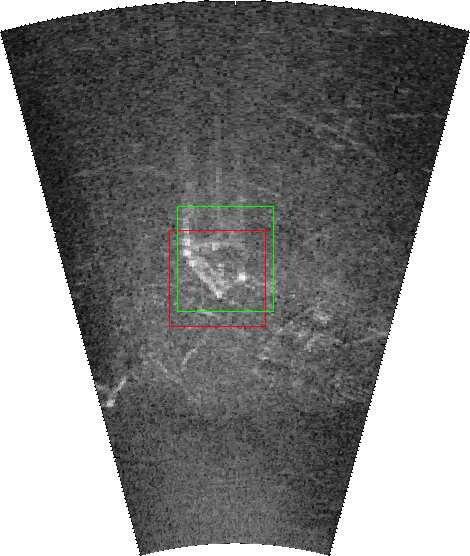
\includegraphics[width=0.30\textwidth]{chapters/images/applications/tracking/2016-02-05_055052-frame02415-proposals.jpg}
        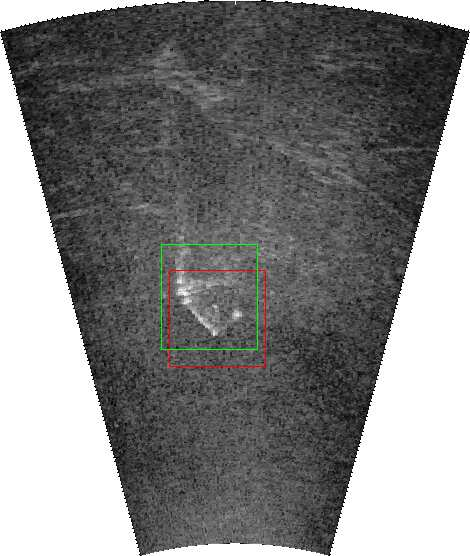
\includegraphics[width=0.30 \textwidth]{chapters/images/applications/tracking/2016-02-05_055052-frame02442-proposals.jpg}
        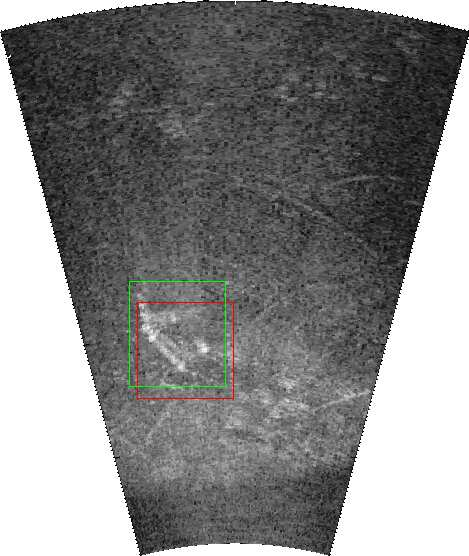
\includegraphics[width=0.30 \textwidth]{chapters/images/applications/tracking/2016-02-05_055052-frame02462-proposals.jpg}
    }
    
    \subfloat[Valve Sequence]{
        \centering
        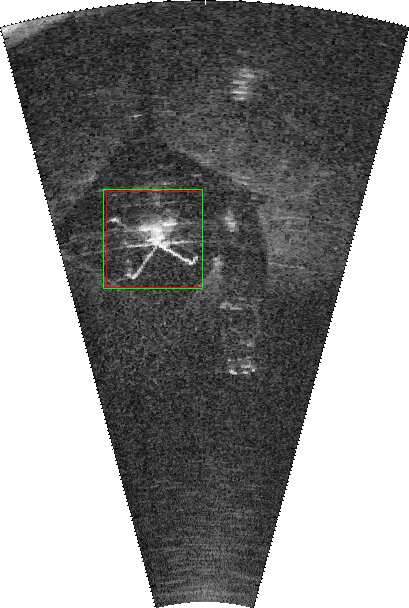
\includegraphics[width=0.23\textwidth]{chapters/images/applications/tracking/2016-02-11_070611-frame16017-proposals.jpg}
        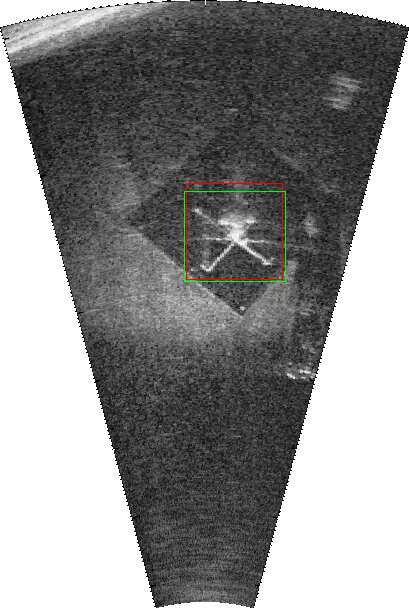
\includegraphics[width=0.23\textwidth]{chapters/images/applications/tracking/2016-02-11_070611-frame16046-proposals.jpg}
        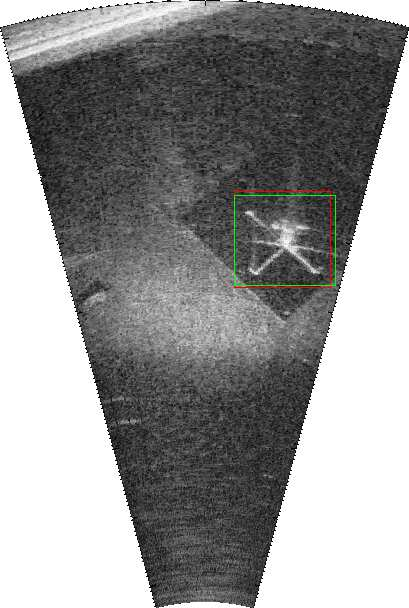
\includegraphics[width=0.23\textwidth]{chapters/images/applications/tracking/2016-02-11_070611-frame16070-proposals.jpg}
    }
    
    \subfloat[Bottle Sequence]{
        \centering
        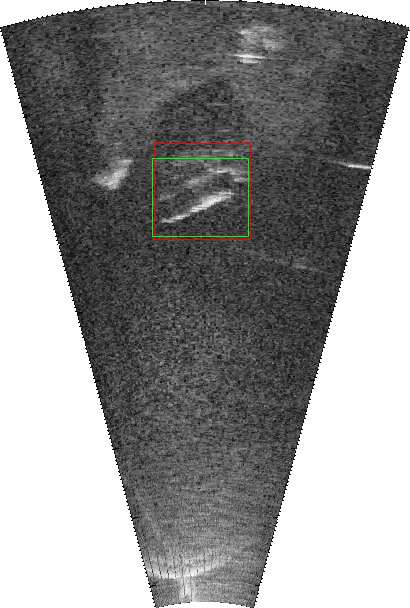
\includegraphics[width=0.23\textwidth]{chapters/images/applications/tracking/2016-02-11_070611-frame02632-proposals.jpg}
        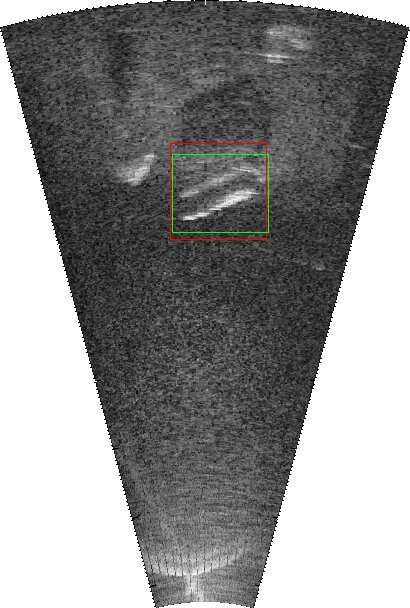
\includegraphics[width=0.23\textwidth]{chapters/images/applications/tracking/2016-02-11_070611-frame02640-proposals.jpg}
        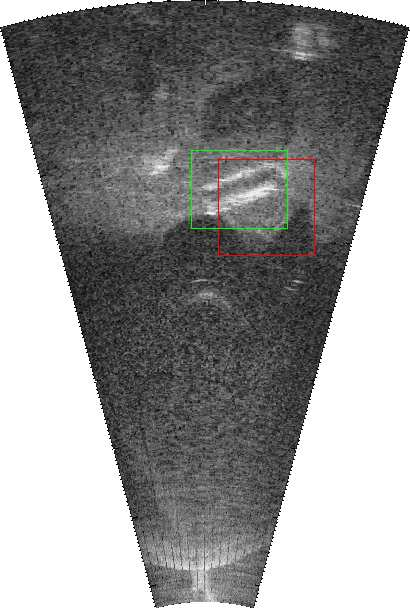
\includegraphics[width=0.23\textwidth]{chapters/images/applications/tracking/2016-02-11_070611-frame02681-proposals.jpg}
    }
    \vspace*{0.5cm}
    \caption[Sample tracking results generated by our tracker]{Sample tracking results generated by our tracker. Green is the ground truth, while red is the bounding box generated by our tracker.}
    \label{sampleTrackerFrames}
\end{figure*}